\section{Tipo de algoritmos de Machine Learning}
\label{sec:ml-types}

Existem diferentes tipos de algoritmos de aprendizagem, os principais são: \textbf{aprendizagem supervisionada}, \textbf{aprendizagem não-supervisionada},
\textbf{aprendizagem semi-supervisionada} e \textbf{aprendizagem por reforço}, onde segundo ~\cite{uso_ml} extima-se que 70\% dos algoritmos de aprendizagem são de 
aprendizagem supervisionada, e algo entre 10\% e 20\% são não-supervisionada, enquanto o restante são os menos utilizados.
\subsection{Aprendizagem supervisionada}
\label{subsec:supervised-learning}
Este tipo de algoritmo é utilizado quando a informação a ser utilizada para predição esta presente nos dados de treino, chamados de 
exemplos rotulados. Por exemplo um conjunto de dados de transações que possui um attributo que diz se é uma transação fraudulenta, o 
algoritmo procurará um padrão destes marcados como fraudulentos e gerará um modelo que indique a probabilidade de uma nova transação 
ser fraudulenta.

Aprendizagem supervisionada é mais apropriada e mais usada em aplicações que utilizão dados historicos para realizar predições. 
Basicamente utiliza-se padrões de dados rotulados para predizer novos dados não rotulados. 
Os métodos mais utilizados são \textbf{classificação}, \textbf{regressão} ou \textbf{predição numérica}.

O principal objetivo da aprendizagem supervisionada é construi um classificador que possa identificar a classe de novos dados apartir
do treinamento em exemplos rotulados.     


\subsubsection{Classicação}
\label{subsubsec:classificacao}

Classicação é um método que tem como objetivo categorizar novos dados em classes baseadas em atributos discretos ou qualitativo,
por exemplo um atributo é discreto quando assume um valor numérico de um conjunto finito de número ou uma quantidade enquanto que um
atributo qualitativo representa uma categoria como o sexo de uma pessoa podendo assumir o valor masculino ou feminino.
Em suma os novos dados são categorizados com base nas classes dos dados de treinamento (exemplos rotulados). 
Mas para que se possa estimar qual a classe destes novos dados é preciso de um \textbf{classificador},
este é o produto de um \textbf{indutor}, o objetivo de um indutor é extrair o melhor classificador possível de um dado 
conjunto de exemplos rotulados.
Um classificador é gerado após exemplos rotulados serem submetidos á um dado indutor, após a geração do classificador 
é necessário identificar a qualidade do mesmo, apartir de métricas pré-definidas até atingir resultados aceitáveis, após a aceitação do classificador 
serão submetidos exemplos não rotulados e o classificador deverá enquadrar os dados em suas devidas classes com precisão. 
\begin{figure}[htb!]
	\centering
	\Caption{\label{fig:novo-classificador} Processo geração do classificador}	
	\UECEfig{}{
		\fbox{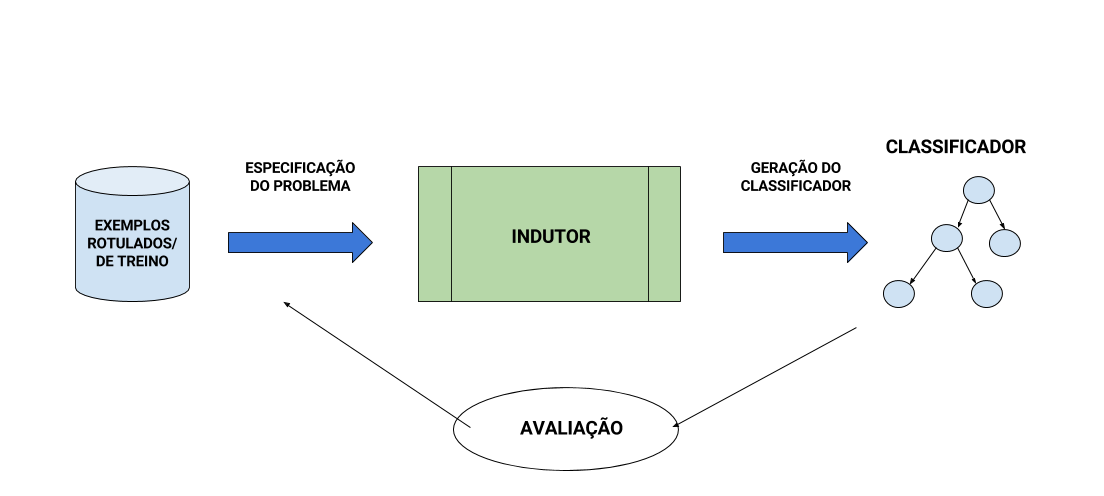
\includegraphics[width=14cm]{figuras/n-classifier}}
	}{
		\Fonte{Autoria própria}		
	}	
\end{figure}  

A Figura ~\ref{fig:amostra-transacoes} ilustra o exemplo de transações de cartão de crédito fraudulentas, dado que tem-se uma 
amostra de transações realizadas. Após estes dados serem submetidos ao classificador, irá predizer com um dado grau de probabilidade 
a qual classe o exemplo pertence, logo sua saída basicamente será como aprensentado na Figura ~\ref{fig:amostra-transacoes-classefied}:
\begin{figure}[ht!]
	\centering
	\Caption{\label{fig:amostra-transacoes} Amostra de Transações de cartão de crédito}	
	\UECEfig{}{
		\fbox{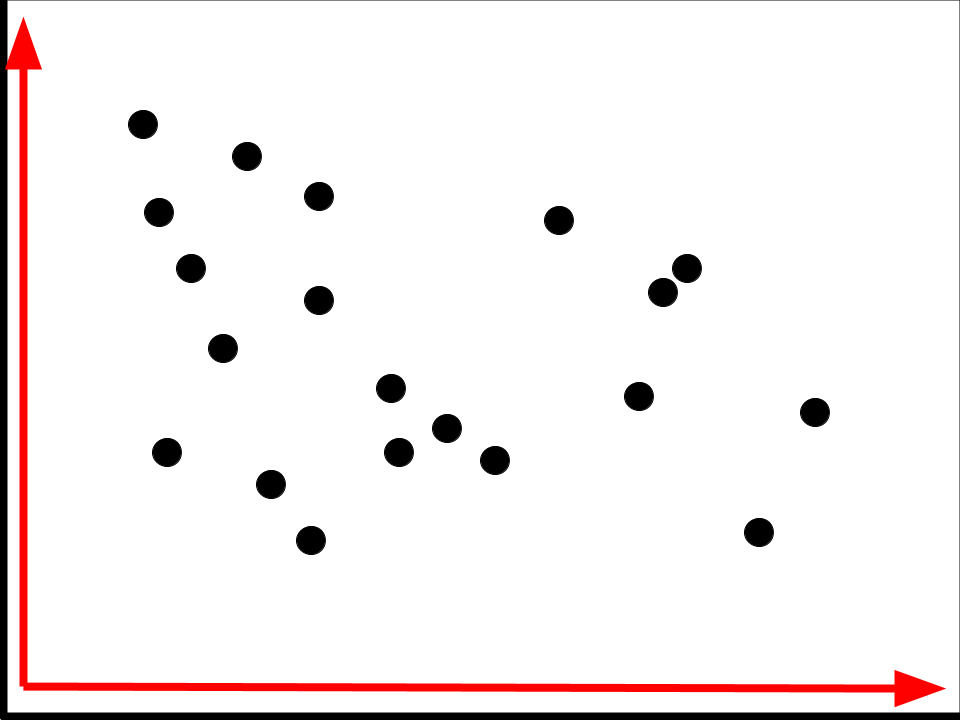
\includegraphics[width=8cm]{figuras/dados-nao-classificados}}
	}{
		\Fonte{Autoria própria}		
	}	
\end{figure}
\begin{figure}[ht!]
	\centering
	\Caption{\label{fig:amostra-transacoes-classefied} Amostra de Transações de cartão de crédito classificadas}	
	\UECEfig{}{
		\fbox{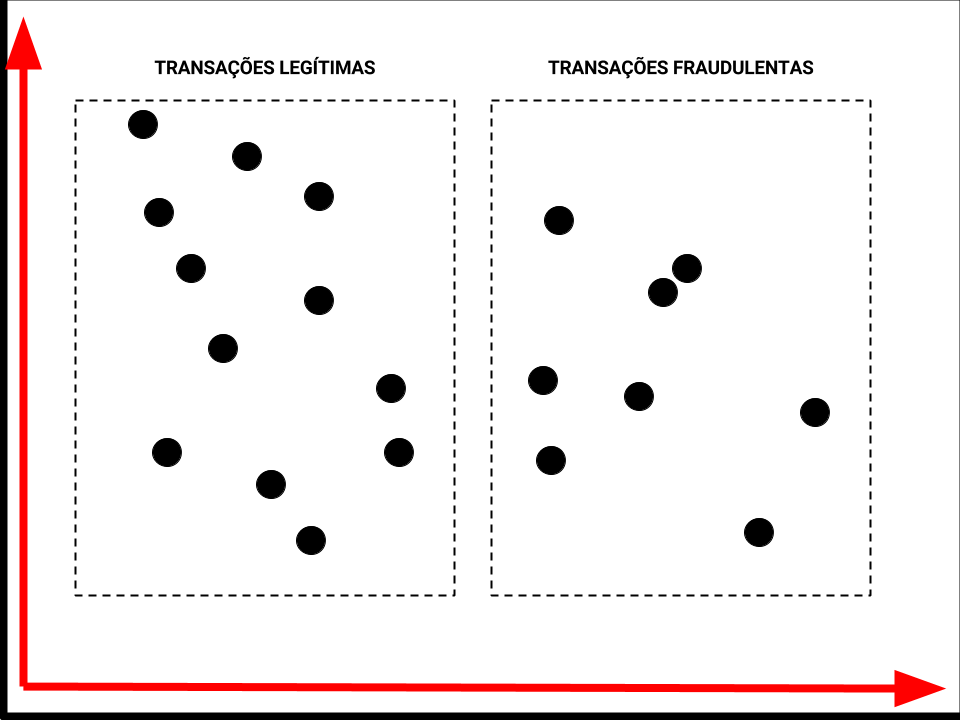
\includegraphics[width=8cm]{figuras/dados-classificados}}
	}{
		\Fonte{Autoria própria}		
	}	
\end{figure}

Existem alguns algoritmos de classificação muito utilizados como  \textbf{árvore de decisões} e \textbf{classificação por regras}.


\subsubsection{Classificação com Árvore de decisões}
\label{subsubsec:decision-tree}
Este algoritmo tem com objetivo particionar em classes de forma recursiva os exemplos rotulados, é importante lembrar que este método
utiliza tanto atributos discretos quanto recursivos para classificar. Alguns algoritimos como ID3, ASSISTANT, CART E C4.5 
são utilizados para construção destas árvores de decisão.

Árvores de decisão são facilmente representadas por um fluxograma com a estrutura de uma árvore, onde o ponto de partida é chamado de nó raiz,
além do nó raiz temos os nós terminais e não terminais também conhecidos como ramos e folhas. Posto que os nós não-terminais/ramos se divide em nós filhos,
e está divisão é dada por uma condição sobre o valor de um atributo de um exemplo, enquanto que os nós terminais/folhas não se dividem, ele atribui uma classe ao exemplo.

Dado uma árvore de decisão utilizada para classificar pacientes doentes e saudáveis:

\begin{figure}[ht!]
	\centering
	\Caption{\label{fig:ex-arvore} Exemplo árvores de decisão }	
	\UECEfig{}{
		\fbox{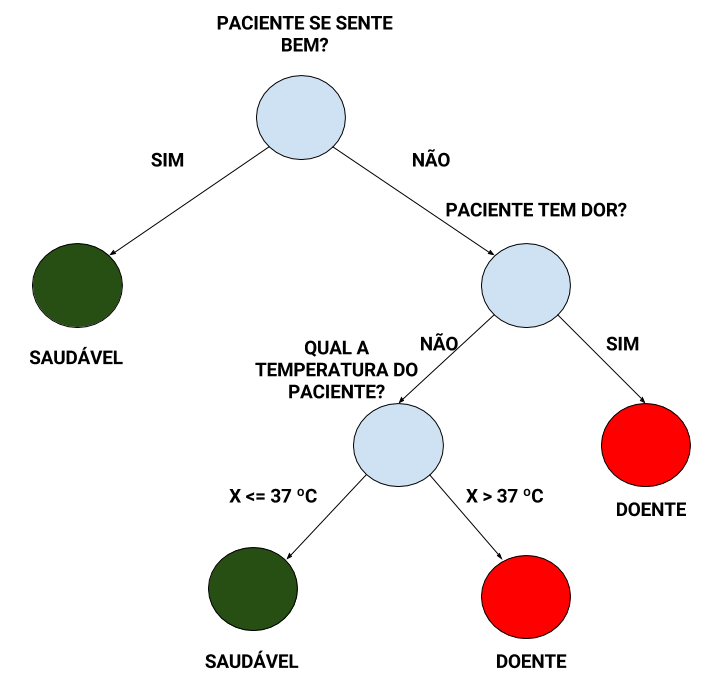
\includegraphics[width=12cm]{figuras/ex-arvore-decisao}}
	}{
		\Fonte{Autoria própria}		
	}	
\end{figure}

Ao submeter um conjunto de dados de uma paciente com os seguintes atributos \{Se sente bem: Sim, Paciente Sente Dor: Não, Temperatura: 38\}, 
este exemplo será classificado como doente por conta das regras aplicadas durante o fluxo.

\subsubsection{Regressão}
\label{subsubsec{regressao}}
Regressão assim como em classicação utiliza de exemplos rotulados para treino, porém estes rótulos são baseados em atribudos com valores contínuos, 
diz-se que um atributo é contínuo quando assume qualquer valor numéricos presente em um conjunto infinito em uma determinada escala, por exemplo o preço de uma casa, 
pode ser R\$300.000,00 ou R\$890.092,00. Seu objetivo é identificar um modelo de curva ou uma função linear \textit{y = f(x)}, com base
em parâmetros conhecidos dos exemplos de treino, para prever o valor do \textbf{rótulo} em novos dados.
Por exemplo dado um conjunto de dados de treino que diz respeito à um imóvel, pretende-se identificar um modelo para poder predizer
o preço de imóveis:

\begin{table}[h!]
	\Caption{\label{dados-imoveis} Exemplos rotulado de dados de imóveis}
	\IBGEtab{}{
		\begin{tabular}{rr}
			\toprule
			Área ($m^{2}$) & Preco (R\$) \\
			\midrule \midrule
			192,00  &        250.000,00  \\
			140,55  &        187.000,00  \\
			88,90   &         88.590,00  \\
			73,82   &         69.000,00  \\
			125,50  &        120.456,00  \\
			110,80  &        108.459,00  \\
			400,90  &        800.750,00  \\
			399,90  &        780.000,00  \\
			\bottomrule
		\end{tabular}
	}{
    \Fonte{Produzido pelo autor}
	\Nota{A coluna preço é o rótulo de cada exemplo.}	
}
\end{table} 

Pretende-se identificar um modelo que ao aplicar um novo imóvel com área de \textit{x $m^2$} me retorne o seu possível valor. A Figura ~\ref{fig:regressao-plano-cartesiano} ilustra 
o modelo de regressão deste caso, que é basicamente um função linear \textit{y = f(x)}, onde \textbf{\textit{y}} seria o valor que estamos tentando inferir e \textbf{\textit{x}} é o parâmetro 
conhecido que será utilizado, neste caso a área do imóvel.

\begin{figure}[ht!]
	\centering
	\Caption{\label{fig:regressao-plano-cartesiano} Exemplo Regressão}	
	\UECEfig{}{
		\fbox{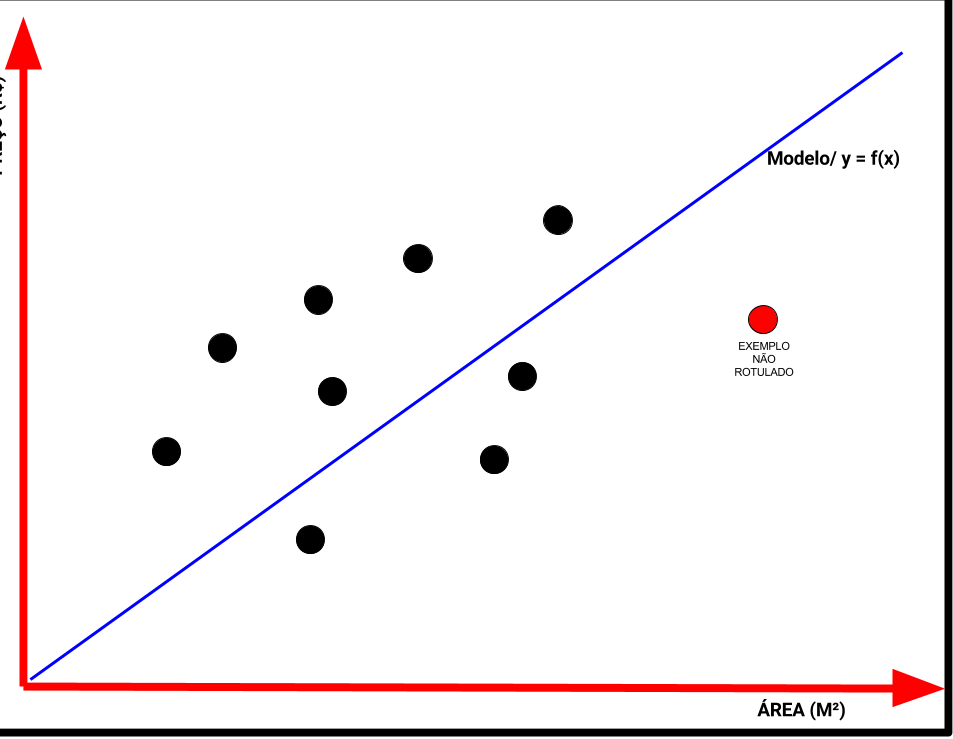
\includegraphics[width=12cm]{figuras/regressao-plano-predicao-imovel}}
	}{
		\Fonte{Autoria própria}		
	}	
\end{figure}
\subsection{Aprendizagem não-supervisionada}
\label{subsec:unsupervised-learning}

Diferente de aprendizagem supervisionada, este método não conta com dados históricos rotulados. Em suma tem como objetivo encontrar
uma forma de estruturar ou organizar estes dados em grupos consistentes. Com este agrupamento feito é possível identificar 
as diferenças e similaridades entre eles e com isso extrair alguns 
\textit{insights}\footnote{ \cite{insight} Insight é um substantivo com origem no idioma inglês e que significa 
compreensão súbita de alguma coisa ou determinada situação.}.

Aprendizagem não-supervisionada utiliza a técnica de clusterização para agrupar grandes quantidades de dados não rotulados,
e após identificar estes grupos criar rótulos para identificar padrões em novos dados e agrupá-los no seu respectivo
grupo.

\subsubsection{Clusterização}
\label{subsec:clustering}
O principal conceito utilizado na técnica de clusterização é o \textbf{\textit{cluster}} que é um conjunto de dados similares.
Logo clusterização é o agrupamento de dados em clusters. Este método de aprendizagem não-supervisionada é aplicada em muitas áreas
pela sua caracteristica de poder identificar \textit{clusters} por similaridades não explicítas, logo é possível retirar informações
de negócio muito úteis. Como por exemplo identificar grupos de clientes e desenvolver ações de \textit{marketing} direcionadas
para cada grupo, ou em empresas de seguros onde é importante identificar os riscos que um cliente oferece e assim estimar o
custo da apólice.

Uma boa clusterização deve gerar clusters com alta similaridade entre seus exemplos e baixa similaridade entre si. A qualidade 
dos resultados dependem da medida de similaridade usada e do \textbf{método} de clusterização e sua implementação,
a qualidade do método também pode ser mediada pela capacidade de identificar padrões escondidos entre os dados.

A qualidade de um cluster é dada pela medida de proximidade entre objetos de um mesmo cluster, em outras palavras a medida de 
proximidade indica a similaridade entre os objetos. A proximidade entre dois objetos \textit{x} e \textit{y} é dada pela função
de distância \textit{d(x,y)}, um objeto é um exemplo, logo ele possui atributos e existe uma função de 
distância para cada tipo de atributo. São os tipos:

\begin{alineas}
	\item \textbf{Numéricos}: como por exemplo: temperatura, latitude, idade, altura, peso, etc.; 
	\item \textbf{Binários}: possuem somente dois estados por exemplo, 1 ou 0, homem ou mulher, verdadeiro ou falso, etc.; e
	\item \textbf{Nominais}: basicamente é um generalização do tipo \textbf{binário}, por exemplo tipos de filmes(ação, aventura, comédia, romance, etc..).  
\end{alineas}

A seleção de atributos para clusterização é uma etapa muito importante pois deve-se ter uma preocupação em escolher os atributos
que representem a maior quantidade informação possível sobre a finalidade do projeto. Também existe uma procupação com a redundância
entre estes atributos a qual deve ser mínima.

Dado o problema que a aprendizagem deseja resolver, alguns atributos terão mais pesos que outros como uma têndencia, que deverá influenciar
diretamente na formação dos clusteres, isto é chamdo de \textbf{critério de agrupamento}, este critério é normalmente definido por um especialista.

Após a definição da medida de proximidade e o critério de agrupamento, é necessário identificar qual algoritmo de clusterização utilizar.
Basicamente estes algoritmos pretendem identificar padrões nos dados. Estes podem ser divididos em categorias, suas principais são:

\begin{alineas}
	\item \textbf{Sequenciais}: são diretos e rápidos, e normalmente os mesmos dados passam várias pelo algoritmo e a ordem em que os 
	dados são submetidos ao algoritmo influencia diretamente no resultado. Um de seus principais algoritmos é o \textbf{BSAS} (\textit{Basic Sequential Algorithmic Scheme});  
	
	\item \textbf{Hierárquicos}:  é dividido em duas subcategorias:
		\begin{alineas}
			\item \textbf{Aglomerativos}: a cada iteração diminui a quantidade de clusters como a ~\autoref{fig:proc-aglo} ilustra, fundindo o cluster da iteração anterior com a atual; e 
			\item \textbf{Divisivos}, a cada iteração almenta a quantidade de clusters como a ~\autoref{fig:proc-div}, dividindo o cluster em 2. 
		\end{alineas} 	
	\item \textbf{Baseados em otimização}: utiliza diversas técnicas de cálculo para otimização de uma função de custo \textit{J}, 
	onde o custo \textit{J} é uma função de vetores\footnote{Vetor é um conjunto de atributos de um exemplo} de um conjunto de exemplos \textit{X} e é parametrizado em termos de um 
	vetor de parâmetros desconhecidos. O objetivo é estimar os parâmetros desconhecidos que melhor caracterize os clusters no
	conjunto de dados. Existem três principais subcategorias de algoritmos:  
	\begin{alineas}
		\item \textbf{Decomposição de misturas}: a função de custo é baseada em atributos aleatórios;
		
		\item \textbf{Método \textit{Fuzzy}}: é definida uma função de proximidade entre um vetor e um cluster e o
		 “grau de afiliação (adesão)” de um vetor a um cluster é fornecido por um conjunto de funções afiliação; e	
		
		\item \textbf{Método \textit{Hard}}: cada vetor pertence exclusivamente a um único cluster, por este motivo é chamado de \textit{Hard}.		 	
	\end{alineas} 		
\end{alineas}   

O algoritmo mais usado para clusterização é o \textbf{K-Means}, e é usado como base para vários outros algoritmos.
Como dito por \cite{k-means}, o algoritmo \textit{k-means} evoluiu ao longo do tempo, existem muitas implementações do algoritmo.
 
 O entendimento deste algoritmo possibilita uma fácil assimilação de  muitos outros algoritmos de clusterização usados atualmente,
 apesar destes algoritmos terem avançado muito desde a criação do k-means, não quer dizer que seja obsoleto,  
 o ~\autoref{qua:k-means-str-wek} mostra algumas caracteristicas deste algoritmo.

 O algoritmo \textit{k-means} relaciona cada exemplo em um dos \textit{k} clusters, onde \textit{k} é a quantidade de clusters 
 especificada previamente. Tem como objetivo minimizar a diferença entre os membros do cluster e aumentar a diferença entre os clusters.
 Se a quantidade de exemplos e quantidade de clusters não forem muito pequenas, não é praticável encontrar os melhores clusters dentre 
 todas as combinações possíveis de exemplos. Por isso ele utiliza de heurística, logo o algoritmo inicia com um palpite para 
 formação dos clusters, depois modifica os relacionamentos suavemente para que possa verificar se a homogeneidade dos elementos
 dos clusters melhorou. Este processo acontece muitas vezes até que as alterações não surtam mais efeito, quando isto ocorre os
 clusters são finalizados. 
 
 \begin{figure}[ht!]
	\centering
	\Caption{\label{fig:proc-aglo} Iterações algoritmos aglomerativos}	
	\UECEfig{}{
		\fbox{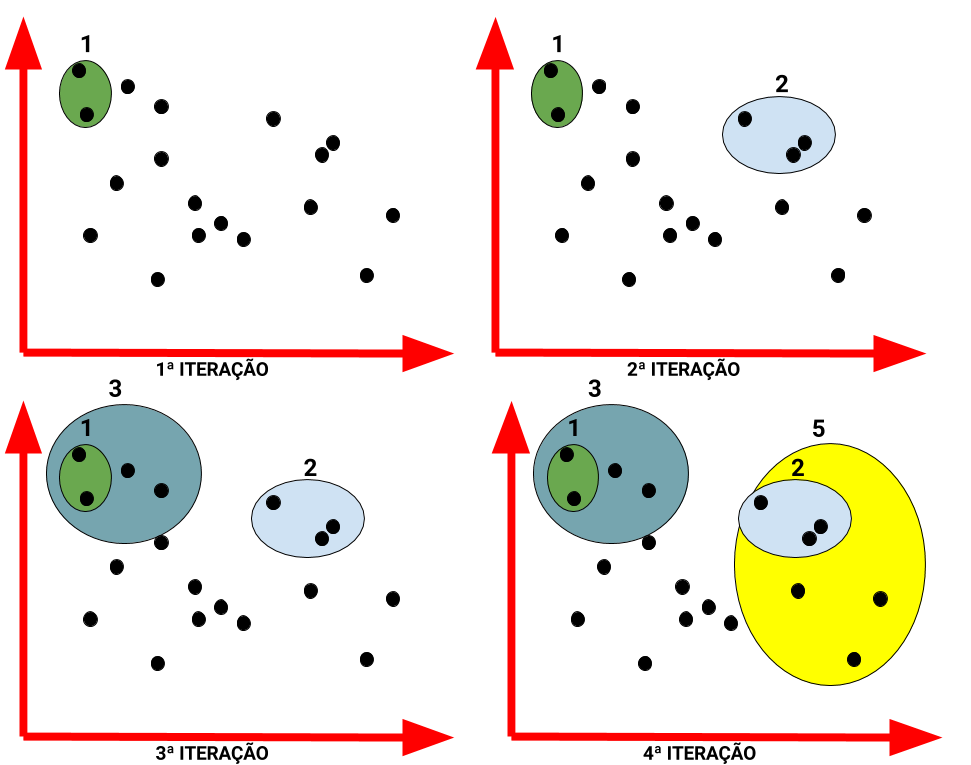
\includegraphics[width=12cm]{figuras/processo-aglomerativo}}
	}{
		\Fonte{Autoria própria.}		
	}	
\end{figure}
\begin{figure}[ht!]
	\centering
	\Caption{\label{fig:proc-div} Iterações algoritmos divisivos}	
	\UECEfig{}{
		\fbox{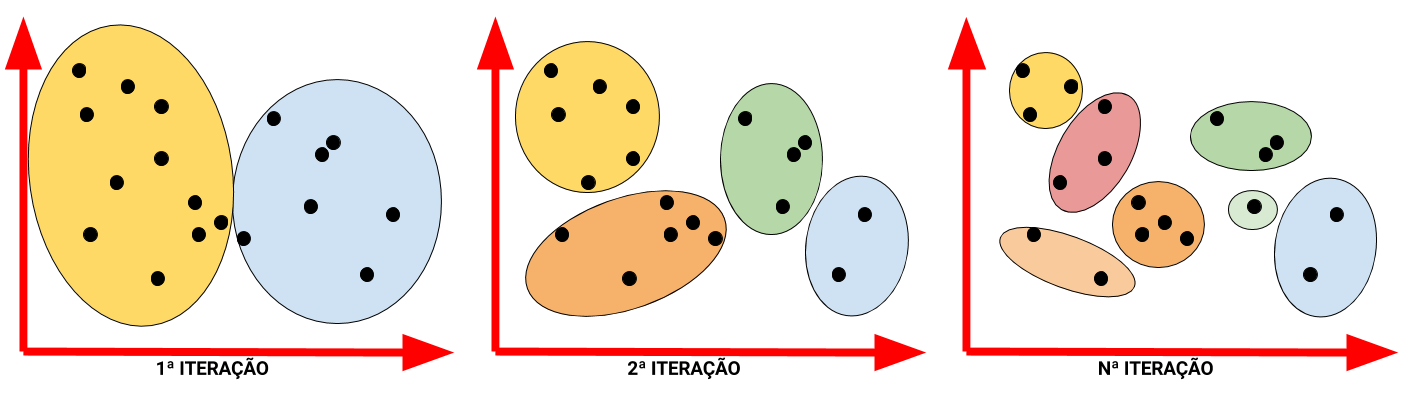
\includegraphics[width=14cm, height=4cm]{figuras/processo-divisivo}}
	}{
		\Fonte{Autoria própria.}		
	}	
\end{figure}

\begin{quadro}[h!]	
	\centering
	\Caption{\label{qua:k-means-str-wek} Vantagens e Desvantagens Algoritmo k-means}		
	\UECEqua{}{
		{\renewcommand{\arraystretch}{2}
		\begin{tabular}{|L{7cm}  L{7cm}|}
			\hline
			Vantagens & Desvantagens \\
			\hline
			\tabitem Utiliza principios simples para identificar \textit{clusters}, quais podem ser explicados
			em termos não estatísticos.
			
			
			\tabitem  É altamente flexísivel e tem a capacidade de se adaptar e com poucos ajustes sanar suas deficiências.
			
			
			\tabitem É muito eficiente e separa os dados em clusters uteis.		
			& 
			\tabitem É menos sofisticado que os algoritmos de clusterização mais recentes.


			\tabitem Por usar elementos aleatórios para treino, não há garantia de encontrar os melhores \textit{clusters}.
			
			
			\tabitem Requer um parâmetro assertivo sobre a quantidade de clusters existentes no conjunto de dados. 
			\\
			\hline
		\end{tabular}
		}
	}{
		\Fonte{Autoria própria.}
	}
\end{quadro}

\subsection{Aprendizagem Semi-Supervisionada}
\label{subsec:semi-supervised-learning}
Esta categoria como o próprio nome sugere é uma mistura entre aprendizagem supervisionada e não-supervisionada, 
esta mistura se dá por utilizar tanto exemplos rotulados como exemplos não rotulados para treino, na maiorias dos casos se utiliza 
mais dados não rotulados do que rotulados, isto porque é mais barato e mais fácil de adquiri-los. É útil quando o processo de preparação
dos dados é muito custoso para realizar treino com exemplos  rotulados.
Alguns dos exemplos que utilizam este tipo e aprendizagem é reconhecimento de fala e de rostos, justamente pela variedade
de formas de rostos, dicção ou sotaques diferentes.

Dado que temos \textit{L} e \textit{U} sendo a quantidade exemplos rotulados e sem rótulos, temos $X_{1:L}$ e $X_{L+1: L+U}$ como vetores de atributos dos exemplos
rotulados e não rotulados respectivamente e o rótulo $y_{1:L}$.  O objetivo de um algoritmo semi-supervisionado é definir 
um classificador $f : x \rightarrow y$ com base em exemplos rotulados e não-rotulados. Existem dois paradigmas que a aprendizagem
semi-supervisionado utiliza, são eles:

\begin{alineas}
	\item \textbf{Aprendizagem Transdutiva\footnote{Transdutivo é a ligação de fatos que não mantêm relação entre si.}}, tem como objetivo aplicar o classificador $f$ somente em exemplos 
	não-rotulados durante o treinamento, e este classificador não generaliza exemplos desconhecidos.\cite{Zhu03semi-supervisedlearning,Zhou04learningwith}
	\item \textbf{Aprendizagem Indutiva}, tem como objetivo identificar um classificador $f$, que pode ser aplicado em exemplos desconhecidos.
	\cite{indutive-learning} 
\end{alineas} 
\subsection{Aprendizagem por reforço}
\label{subsec:reforcing-learning}
 
Muito semelhante a tradicional análise de dados onde o algoritmo de descoberta por tentativa e erro
decide qual ação resulta em maior ganho, e diferente dos outros métodos de aprendizagem não utiliza exemplos para treino
e sim trabalha com feedbacks do ambiente. de acordo com \cite{Valiant:1984:TL:1968.1972} "O número de exemplos necessários para 
se aprender um certo conceito cresce exponencialmente de acordo com o número de atributos", por isto se utiliza este tipo de aprendizagem
quando o é impraticavel a aprendizagem com exemplos.


Quando se aplicada a aprendizagem por reforço é muito comum utilizar o processo de decisão de Markov (MDP). 
Este tipo de aprendizagem possui três componentes importantes em sua aplicação:
\begin{alineas}
	\item O \textbf{agente}, é o responsável pelas tomadas de decisões.
	\item O \textbf{ambiente}, é tudo com oque o agente interage.
	\item As \textbf{ações}, é oque o agente pode fazer.
\end{alineas}  
 Em suma a aprendizagem por reforço tem como principal objetivo encontra uma política de ações que maximize seus ganhos(recompensa). Para ilustrar 
 pense em um agente em um dado ambiente, onde a cada instante de tempo o agente está:   
\begin{alineascomponto}
	\item em um estado $x$;
	\item executa um ação $a$;
	\item vai para o estado $s'$; e
	\item recebe uma recompensa $r$;
\end{alineascomponto}
Com isso ele consegue coletar informações para identificar qual ação resulta em uma maior recompensa,
está recompensa é um \textit{feedback} do ambiente sobre o comportamento do agente. 
 
De acordo com o MDP tambem conhecido como cadeia de Markov, uma política de ações é dada por $\pi: (S)$
e $\pi: S \rightarrow A $, onde $S$ é um conjunto de estados e $A$ um conjunto de ações. 
O MDP é baseado em dois conceitos fundamentais: \cite{hordijk1992} estados e transições de estado.
Um \textbf{estado} é tido como uma variável aleatória que descreve alguns atributos, é formado por percepções do agente e deve
prover informações para o agente de quais ações podem ser executadas, como por exemplo a quantidade de pessoas em uma festa.
E a \textbf{transição de estado} descreve uma mudança no estado em um período de tempo, 
dado o exemplo da festa uma mudança de estado seria quando a musíca para.

Uma função de recompença é dada por  $r: (S \times A) \rightarrow R$. A função $r(s,a)$ que indica a recompensa 
recebida quando se esta em um estado $s$ e executa uma ação $a$, está pode ser determinística ou estocástica. Logo uma 
função de trasição de estado é dada por $\delta:(S \times A) \rightarrow S $ e $\delta:(s,a)$ que indica em que 
estado um agente está, sendo que estava em um estado $s$ e executou uma ação $a$, em um ambiente não-determinístico
a funça é dada por $\delta:(s,a,s')$ que indica a probabilidade a probabilidade de ir para um estado $s'$ sendo que
estava em um estado $s$ e realizou a ação $a$.
Um bom exemplo de MDP é um agente jogador de Damas como mostra o Quadro ~\ref{qua:agente-jogador}

\begin{quadro}[h!]	
	\centering
	\Caption{\label{qua:agente-jogador} MDP - Agente jogador de damas}		
	\UECEqua{}{
		{\renewcommand{\arraystretch}{2}
		\begin{tabular}{|L{2cm} | L{2cm} | L{2cm}| L{3cm} | L{3cm}|}
			\hline
			Agente & Ambiente & Estados & Ações & Recompensa \\
			\hline
			 Jogador de Damas & Tabuleiro Damas & Posição das peças & Mover uma dada peça & (Capturas de peças - Perdas de peças) \\
			\hline
		\end{tabular}
		}
	}{
		\Fonte{Autoria própria}
	}
\end{quadro}  

A política de ações é responsável por modelar o comportamento de um dado agente mapeando os estados em ações, esta pode 
ser vista como um conjunto de regras tida como $s_{n} \rightarrow a_{n}$, pode ser ilustrada como instruções de controle 
de fluxo \textit{if}, o Algoritmo ~\ref{alg:se} apresenta algumas regras dado o exemplo de um personagem de um jogo:
\begin{algorithm}[h!]
	\SetSpacedAlgorithm
	\caption{\label{alg:se}Exemplo regras política de ações}
	\Entrada{Estado}
	\Saida{Ação}
	\Inicio{
		\Se{estado = (vida em 100\%,energia em 100\%, inimigo ao alcance)}{
			Atacar\;
		}
		\Se{estado = (vida < 50\%, energia em 0\%, inimigo próximo)}{
			Fugir\;
		}
		...\	
	}		
\end{algorithm}   

Posto que uma política de ações mapeia estados em ações, como determinar se um dado estado é bom ou ruim?
A função de valor de estado expressa isto em termos de recompensas e a política de ações, basicamente representa
uma recompensa a receber em um dado estado mais as recompensas futuras se seguir uma certa política de ações, esta
funça é dada por $V\pi(S_{0})= r_{0}+r_{1}+r_{2}+r_{3}+ ... + r_{n}$, é importante atentar para o tempo, pois 
se ele for infinito a função valor tende a infinito. Para garantir a convêrgencia e diferenciar recompensas distantes do
estado atual é utilizado um fator de desconto onde $0 \leqslant \lambda \leqslant 1$  e a função de valor é dada por
$V\pi(S_{t})= r_{t} + \gamma r_{t+1} + \gamma^{2} r_{t+2} + \gamma^{3} r_{t+3} ... \gamma^{n} r_{t+n}$, por exemplo
se o fator $\gamma$ for 90\%, logo a função será:
\begin{equation}
	\begin{aligned}
 			V\pi(S_{t})= r_{t} + 0.9 r_{t+1} + 0.81 r_{t+2} + 0.729 r_{t+3} ... 0.9^{n} r_{t+n}
	\end{aligned}
\end{equation}
Com esta função é possível determinar se um dado estado é bom ou ruim e com isso é possível ter insumos de qual
ações tomar para maximizar a recompensa.